\documentclass{article}
\usepackage{graphicx} % Required for inserting images
\usepackage{url}
\usepackage{amsmath}
\usepackage{subcaption}
\usepackage{algorithm}
\usepackage{algpseudocode}

\title{A Machine Learning Classification Model for Gold-Binding Peptides}
\author{Ali Ahmadi Esfidi}
\date{May 2025}

\begin{document}

\maketitle

\section{Gold-Binding Peptides}
Gold‐binding peptides are short chains of amino acids (typically 5–20 residues) that have a natural affinity for gold surfaces or nanoparticles. They are identified or designed so that specific residues (often cysteine, histidine, or aromatic amino acids) coordinate with gold atoms, allowing the peptide to stick strongly and specifically to gold.\footnote{\url{https://pmc.ncbi.nlm.nih.gov/articles/PMC10337651/}}

\subsection{Usage}
\begin{enumerate}
  \item \textbf{Nano‐templating \& Nanofabrication.} Peptides guide the formation of gold nanowires, rods, or particles with controlled size and shape, serving as a “molecular mold” for electronic or optical devices.\footnote{\url{https://pubs.rsc.org/en/content/articlepdf/2023/ra/d3ra04269c}}
  \item \textbf{Biosensing \& Diagnostics.} When immobilized on electrodes or sensor surfaces, gold‐binding peptides can capture target biomolecules (e.g., antibodies) in a precise orientation, improving sensitivity for medical assays.\footnote{\url{https://pmc.ncbi.nlm.nih.gov/articles/PMC9918321/}}
  \item \textbf{Targeted Drug Delivery \& Imaging.} Conjugating drugs or imaging agents to gold nanoparticles via these peptides allows for targeted delivery and enhanced imaging contrast in cancer or inflammatory disease models.\footnote{\url{https://www.sciencedirect.com/science/article/abs/pii/S0378517324011542}}
  \item \textbf{Surface Functionalization.} They enable simple, one‐step coating of gold surfaces with proteins or other functional polymers, useful in creating antifouling coatings or bioactive interfaces.
\end{enumerate}

\subsection{Intensity}
In spot‐array binding assays, each 10‐residue peptide is immobilized on a solid support and exposed to gold nanoparticles. The \emph{intensity} is defined as the optical (colorimetric) signal measured at each peptide spot, proportional to the amount of bound nanoparticles. Peptides with stronger binding produce darker spots (higher intensity), whereas weak or non‐binding sequences yield lighter spots (lower intensity).

In the dataset of Janairo \emph{et al.}, each of the 1\,720 unique 10‐mer peptides was assigned an intensity value based on the median image‐analysis readout from Tanaka \emph{et al.}'s screen. To classify peptides into binders and non‐binders, the median intensity of the entire set, denoted \(I_{\mathrm{med}}\), was used as the threshold:
\[
I_{\mathrm{med}} = 207{,}500 \quad\text{(arbitrary units)}.
\]
Peptides were then dichotomized into two classes:
\begin{align*}
\text{Class A (strong binders)} &: I > I_{\mathrm{med}}, \\
\text{Class B (weak/non‐binders)} &: I \le I_{\mathrm{med}}.
\end{align*}

Thus, the intensity values (in arbitrary units) provide a relative measure of each peptide’s adsorption of gold nanoparticles under the standardized assay conditions.


\section{Formulation of Problem}
\begin{itemize}
    \item \textbf{Input:}\begin{enumerate}
        \item \textbf{Peptide sequence:} A string of ten amino‐acid letters.

        \item \textbf{Derived features:} Each sequence is converted into a fixed-length numeric vector, so that the model can process it.
    \end{enumerate}

    \item \textbf{Output:} A binary prediction for each input sequence:
    \begin{itemize}
        \item “Strong binder” (class A) if the model believes the peptide’s binding intensity would exceed the threshold set by the median of all measured intensities.
        \item “Weak/non-binder” (class B) otherwise.
    \end{itemize}
\end{itemize}
\subsection{Mathematical Presentation}
\begin{enumerate}
    \item Peptide Sequences:    \[S = \{s_i\},\quad s_i \in \mathcal{A}^{10}\]

    \item Feature Mapping:    \[\forall s_i \in S, \quad \Phi(s_i) = x_i \in \mathbb{R}^d\]
    
    \item Binding Intensities:    \[I = \{I_i\}_{i=1}^N,\quad I_i \in \mathbb{R}_{\ge0},\]

    \item Classification Labels:   \[y_i = 
    \begin{cases}
      A, & I_i > T,\\
      B, & I_i \le T,
    \end{cases}
    \quad T = \mathrm{median}\bigl(\{I_i\}\bigr)\]

    \item Prediction Function: \[
    \forall s_i \in S, \quad
    f(\Phi(s_i)) = \hat y_i \in \{A,B\}
    \]
\end{enumerate}

\subsection{Assumptions}
\begin{enumerate}
  \item All peptides have fixed length 10.
  \item Median intensity threshold $T$ meaningfully separates strong vs.\ weak binders.
  \item Samples are independently and identically distributed.
\end{enumerate}

\section{Dataset}
Dataset comprises 1,720 peptide sequences, which we classify as A or B based on their intensity values.\footnote{\url{https://pubs.acs.org/doi/suppl/10.1021/acsomega.2c00640/suppl_file/ao2c00640_si_001.pdf}}

\subsection{Distribution}
It’s important to confirm class balance before training classifiers, as imbalanced datasets can introduce bias. 

The class sizes are nearly identical; exact count: \textbf{861} for Class A and \textbf{859} for Class B.

However, as illustrated in the violin plot and histogram in Figure 1, Class A peptides are high-intensity binders with intensity values concentrated around 250,000. Class B peptides, conversely, exhibit lower intensity values, ranging widely from nearly 0 to 200,000, and display a prominent left tail.

\begin{figure}[h!]
    \centering
    \begin{subfigure}[b]{0.45\textwidth}
        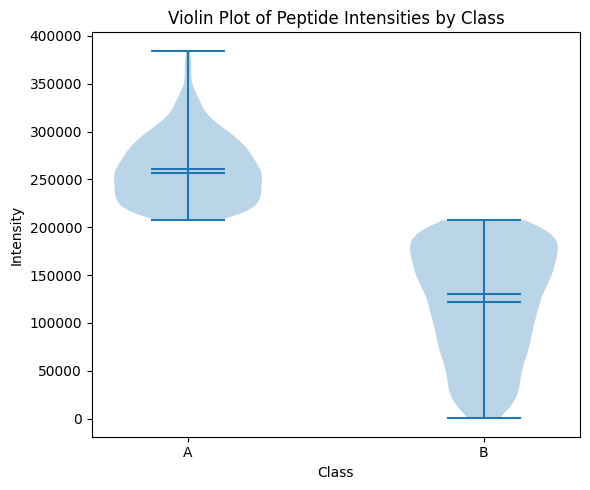
\includegraphics[width=\textwidth]{images/1.png}
        \label{fig:subfig1}
    \end{subfigure}
    \hfill % Adds horizontal space between the subfigures
    \begin{subfigure}[b]{0.45\textwidth}
        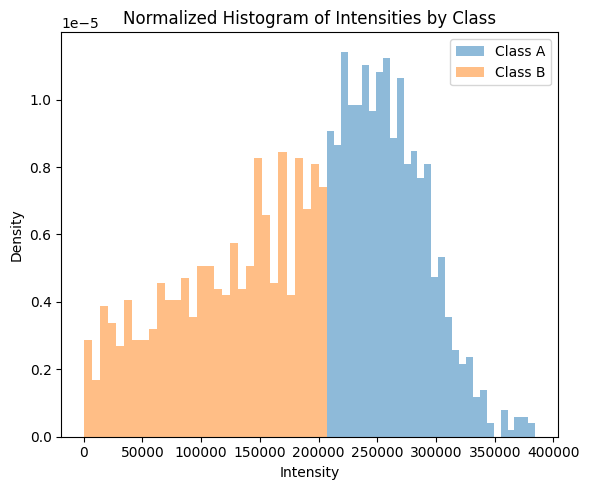
\includegraphics[width=\textwidth]{images/2.png}
        \label{fig:subfig2}
    \end{subfigure}
    \caption{Overall caption for both images.}
    \label{fig:two_images}
\end{figure}

\section{Related Work}
As part of his lecture series, Jose Isagani B. Janairo presents a practical workflow for classifying gold-binding peptides that elegantly demonstrates end-to-end machine-learning in R: starting with raw amino-acid sequences, deriving ten physicochemical descriptors via Kidera factors, and organizing those into a labeled dataset; next, stratified train–validation splitting and 10-fold cross-validation to tune and compare multiple classifiers (logistic regression, decision trees, k-nearest neighbors, SVMs with various kernels, and a neural network); then refining the best performer—a radial-basis SVM—by selecting only the most informative descriptor subset; and finally, assessing generalization on hold-out data and employing permutation-based feature importance to reveal which peptide properties most strongly drive gold-binding predictions, all accompanied by clear visualizations of model performance and variable rankings.

On a macOS environment, the code was executed and produced results (Table 1) consistent with the related lecture (Accuracy: 0.8019).

\begin{table}[h!]
\centering
\begin{tabular}{|c|c|c|}
\cline{2-3}
\multicolumn{1}{c|}{} & \multicolumn{2}{c|}{\textbf{Reference}} \\
\cline{2-3}
\multicolumn{1}{c|}{} & \textbf{A} & \textbf{B} \\
\hline
\textbf{Prediction A} & 175 & 45 \\
\textbf{Prediction B} & 40 & 169 \\
\hline
\end{tabular}
\caption{Confusion Matrix}
\end{table}

Also Table 2 reports the permutation-based importance of each Kidera factor (KF1–KF10) for the final radial‐basis SVM, together with uncertainty bounds and the baseline increase in classification error when that feature is shuffled.

\begin{table}[h!]
\centering
\label{tab:feature_importance}
\begin{tabular}{|c|c|c|}
\hline
\textbf{feature} & \textbf{importance} & \textbf{permutation.error} \\
\hline
KF4 & 1.446512 & 0.2408985 \\
KF2 & 1.395349 & 0.2323780 \\
KF3 & 1.395349 & 0.2323780 \\
KF9 & 1.306977 & 0.2176607 \\
KF10 & 1.158140 & 0.1928737 \\
KF5 & 1.148837 & 0.1913246 \\
KF7 & 1.144186 & 0.1905500 \\
KF6 & 1.130233 & 0.1882262 \\
KF1 & 1.000000 & 0.1665376 \\
KF8 & 1.000000 & 0.1665376 \\
\hline
\end{tabular}
\caption{Feature Importance}
\end{table}

In practice, this tells you that the model heavily relies on KF4, KF2, and KF3—disrupting these degrades performance the most—whereas KF1 and KF8 contribute almost nothing to gold‐binding predictions in the final SVM.

\section{Alternative Models and Embeddings}

To further improve classification performance, we can explore alternative modelling techniques and sequence embedding methods.

\subsection{Modelling Techniques}
\begin{itemize}
    \item \textbf{XGBoost:} A highly optimized implementation of gradient-boosted decision trees. It handles missing values natively, regularizes to prevent overfitting, and often achieves state‑of‑the‑art results on tabular data.
    \item \textbf{Support Vector Machines (SVM):} Effective in high‑dimensional spaces and robust to overfitting when properly regularized. Kernel functions (e.g., RBF, polynomial) allow SVMs to capture non‑linear relationships.
    \item \textbf{Neural Networks:} Neural networks are composed of interconnected layers of artificial neurons that learn hierarchical feature representations directly from input embeddings. By stacking multiple dense or specialized layers and employing non‑linear activation functions (e.g., ReLU, GELU), they can capture complex, non‑linear relationships in the data. Key design considerations include:
\end{itemize}

\subsection{Sequence Embedding Methods}
\begin{itemize}
    \item \textbf{Amino Acid Composition (AAC):} A simple, interpretable feature vector of length 20 that counts the frequency of each amino acid in a peptide or protein.
    \item \textbf{Kidera Factors:} A set of 10 physicochemical descriptors derived via multivariate analysis, summarizing properties like hydrophobicity, bulkiness, and electronic characteristics.
    \item \textbf{BLOSUM62 Encoding:} Using the BLOSUM62 substitution matrix rows as 20‑dimensional vectors for each residue, capturing evolutionary substitution preferences.
\end{itemize}

We concatenate these embeddings to construct a more informative representation of each peptide sequence. The resulting combined embedding is then used as input to the chosen classification model (e.g., XGBoost, SVM, or a neural network). This approach may also reveal the presence of additional discriminative features.

\section{Support Vector Machines (SVM)}
This section details the application of a Support Vector Machine (SVM) classifier. The dataset underwent a rigorous preprocessing sequence to prepare it for model training. First, it was stratified into training and testing sets, ensuring the preservation of the original class distribution. Feature magnitudes were subsequently normalized using \texttt{StandardScaler} to bring them to a common scale. A crucial step involved \textbf{feature selection}, applied to the scaled training data using \texttt{SelectKBest} with the \texttt{mutual\_info\_classif} scoring function. This process identified and retained the most informative features, which were then used to transform both the training and test sets, reducing dimensionality and potential noise. Finally, a Support Vector Machine classifier was trained on these selected features. Its hyperparameters were optimized using \texttt{GridSearchCV} in conjunction with \texttt{StratifiedKFold} cross-validation. The model optimization employed the \textbf{Receiver Operating Characteristic Area Under the Curve (ROC AUC)} as the primary scoring metric, and \texttt{class\_weight='balanced'} was set to effectively address potential class imbalance within the dataset.

\section{XGBoost Classifier}
The combined feature set was subjected to a standard preprocessing workflow for the XGBoost model. Initially, the data was stratified into training and testing sets to preserve the intrinsic class proportions. \textbf{Feature normalization} was then performed using \texttt{StandardScaler}, fitted exclusively on the training data to prevent data leakage. A critical step in this pipeline was \textbf{feature selection}, implemented via \texttt{SelectKBest} with \texttt{mutual\_info\_classif}. This aimed to distill the most relevant features, thereby reducing both dimensionality and potential noise. The core classification model, an XGBoost classifier, was optimized using \texttt{GridSearchCV} with 5-fold cross-validation. The optimization process prioritized the \textbf{ROC AUC} as the primary scoring metric and incorporated the \texttt{scale\_pos\_weight} parameter to effectively address any existing class imbalance.

\section{Residual Attention Classifier}
The data for the Residual Attention Classifier underwent a meticulous preprocessing pipeline. To ensure the preservation of original class distributions, the dataset was initially split into stratified training, validation, and test sets. \textbf{Feature scaling} was subsequently performed using \texttt{StandardScaler}, fitted exclusively on the training data. A key enhancement involved \textbf{feature selection} via \texttt{SelectKBest} with \texttt{mutual\_info\_classif}, which reduced dimensionality and emphasized highly informative features.

A custom \texttt{FeatureDataset} class was developed for PyTorch, enabling on-the-fly \textbf{data augmentation} through the application of Gaussian noise and Mixup. This augmentation strategy was implemented to improve model generalization and robustness. The \texttt{ClassifierNN} architecture integrates several advanced components: \textbf{Residual Blocks} for facilitating deeper network training and mitigating vanishing gradients, \textbf{Attention Pooling} for adaptively weighing feature importance, and \textbf{Exponential Moving Average (EMA)} for achieving more stable model inference. During training, the loss was computed using \texttt{BCEWithLogitsLoss} with \textbf{class weighting} to effectively mitigate class imbalance. The model was optimized using \texttt{AdamW}, a robust optimizer, with a configurable learning rate scheduler (either \texttt{CyclicLR} for cyclical learning rates or \texttt{ReduceLROnPlateau} for adaptive learning rate reduction). Additionally, \textbf{early stopping} was employed to prevent overfitting, and \textbf{gradient clipping} was applied to maintain training stability.

\begin{algorithm}
\caption{Residual Attention Architecture}
\begin{algorithmic}[1]
\Statex
\Function{ResidualBlock}{$x, \text{in\_dim}, \text{out\_dim}, \text{dropout\_rate}$}
    \State $\text{id} \gets \text{x}$
    \State $h \gets \text{Swish}(\text{BatchNorm}(\text{Linear}_1(x)))$
    \State $h \gets \text{Dropout}(h)$
    \State $h \gets \text{BatchNorm}(\text{Linear}_2(h))$
    \State \Return $\text{Swish}(h + \text{id})$
\EndFunction
\Statex
\Function{AttentionPooling}{$x$}
    \State $s \gets \text{Linear}_2(\text{Tanh}(\text{Linear}_1(x)))$ \Comment{Attention scores}
    \State $\alpha \gets \text{softmax}(s)$ \Comment{Feature weights}
    \State \Return $x \odot \alpha$ \Comment{Element-wise multiplication}
\EndFunction
\Statex
\Function{ClassifierNN}{$x$}
    \State $h_0 \gets \text{Linear}_{\text{proj}}(x)$ \Comment{Initial projection}
    \State $h_{i+1} \gets \text{ResidualBlock}(h_i)$
    \State $y \gets \text{AttentionPooling}(h_a)$
    \State \Return $\text{Linear}_{\text{out}}(y)$ \Comment{Binary classification output}
\EndFunction
\end{algorithmic}
\end{algorithm}

\section{Siamese-like Classifier}
The Siamese-like Classifier pipeline commenced by independently loading and processing three distinct types of amino acid sequence embeddings: \texttt{iFeature AAC}, \texttt{Kidera}, and \texttt{BLOSUM62}. Consistency of the target variable was ensured across these diverse datasets. The data for each embedding type then underwent a meticulous preprocessing pipeline, involving \textbf{stratified splitting} into training, validation, and test sets to maintain class proportions. This was followed by \textbf{feature scaling} using \texttt{StandardScaler}, fitted exclusively on the respective training data for each embedding. A critical step was the application of \texttt{SelectKBest} with \texttt{mutual\_info\_classif} for \textbf{feature selection}, aiming to reduce dimensionality and focus on highly informative features specific to each embedding type.

The implementation leveraged a custom \texttt{FeatureDataset} for PyTorch, which supported on-the-fly \textbf{data augmentation} techniques such as Gaussian noise and Mixup to further enhance model generalization. The core \texttt{SiameseClassifier} architecture employed separate \texttt{EmbeddingBranch} networks for each embedding type. This design allowed each branch to learn distinct, specialized representations from its respective input. The outputs of these branches were then concatenated into a shared classification head. Each \texttt{EmbeddingBranch} incorporated \textbf{SiLU activation functions}, \textbf{BatchNorm1d} for improved training stability, and \textbf{Dropout layers} for regularization. The overall model was optimized using \texttt{AdamW}, with a configurable learning rate scheduler (\texttt{CyclicLR} or \texttt{ReduceLROnPlateau}).

During training, \texttt{BCEWithLogitsLoss} with \textbf{class weighting} was utilized to address inherent class imbalance. Furthermore, \textbf{early stopping} was implemented to prevent overfitting, and \textbf{gradient clipping} was applied to ensure training stability. The weights of the best-performing model, as determined by the validation metric, were saved using an \texttt{EarlyStopping} mechanism.

\begin{algorithm}
\caption{Siamese-like Architecture}
\begin{algorithmic}[1]
\Statex
\Function{EmbeddingBranch}{$x, \text{input\_dim}, \text{out\_dim}, \text{dropout\_rate}$}
    \State $x_{i+1} \gets \text{Dropout}(\text{SiLU}(\text{BatchNorm}(\text{Linear}(x_{i}))))$
    
    \State $x_a \gets \text{Linear}(x_a)$
    \State $x_a \gets \text{BatchNorm}(x_a)$
    \State \Return $\text{SiLU}(x_a)$
\EndFunction
\Statex
\Function{SiameseClassifier}{$x_{\text{aac}}, x_{\text{kidera}}, x_{\text{blosum}}$}
    \State $\text{emb}_{\text{aac}} \gets \text{EmbeddingBranch}(x_{\text{aac}})$
    \State $\text{emb}_{\text{kidera}} \gets \text{EmbeddingBranch}(x_{\text{kidera}})$
    \State $\text{emb}_{\text{blosum}} \gets \text{EmbeddingBranch}(x_{\text{blosum}})$
    \State $c \gets \text{Concat}(\text{emb}_{\text{aac}}, \text{emb}_{\text{kidera}}, \text{emb}_{\text{blosum}})$
    \State $h \gets \text{Linear}(c, \text{dim}_{c}/2)$
    \State $h \gets \text{BatchNorm}(h)$
    \State $h \gets \text{SiLU}(h)$
    \State $h \gets \text{Dropout}(h)$
    \State \Return $\text{Linear}(h)$
\EndFunction
\end{algorithmic}
\end{algorithm}

\section{Results}
This section presents the performance of the various machine learning models employed for classifying gold-binding peptides. The evaluation metrics include Accuracy, F1-score (for both classes and macro average), Precision, Recall, and ROC AUC, alongside their respective confusion matrices.

\subsection{XGBoost Classifier Performance}
The XGBoost classifier demonstrated strong performance on the test set.

The confusion matrix for the XGBoost model is presented in Table \ref{tab:xgboost_cm}.

\begin{table}[h!]
\centering
\begin{tabular}{|c|c|c|}
\hline
 & \multicolumn{2}{c|}{\textbf{Reference}} \\
\cline{2-3}
 & \textbf{Class B} & \textbf{Class A} \\
\hline
\textbf{Prediction Class B} & 169 & 46 \\
\hline
\textbf{Prediction Class A} & 32 & 183 \\
\hline
\end{tabular}
\caption{Confusion Matrix for XGBoost Classifier}
\label{tab:xgboost_cm}
\end{table}

\subsection{Support Vector Machine (SVM) Classifier Performance}
The Support Vector Machine (SVM) classifier achieved notable results, exhibiting high overall accuracy and balanced F1-scores.

The confusion matrix for the SVM model is presented in Table \ref{tab:svm_cm}.

\begin{table}[h!]
\centering
\begin{tabular}{|c|c|c|}
\hline
 & \multicolumn{2}{c|}{\textbf{Reference}} \\
\cline{2-3}
 & \textbf{Class B} & \textbf{Class A} \\
\hline
\textbf{Prediction Class B} & 176 & 39 \\
\hline
\textbf{Prediction Class A} & 35 & 180 \\
\hline
\end{tabular}
\caption{Confusion Matrix for SVM Classifier}
\label{tab:svm_cm}
\end{table}

\subsection{Residual Attention Neural Network Performance}
The Residual Attention Neural Network delivered a strong performance, achieving the highest accuracy among the single-embedding models.

The confusion matrix for the Residual Attention Neural Network is presented in Table \ref{tab:residual_attention_cm}.

\begin{table}[h!]
\centering
\begin{tabular}{|c|c|c|}
\hline
 & \multicolumn{2}{c|}{\textbf{Reference}} \\
\cline{2-3}
 & \textbf{Class B} & \textbf{Class A} \\
\hline
\textbf{Prediction Class B} & 171 & 44 \\
\hline
\textbf{Prediction Class A} & 28 & 187 \\
\hline
\end{tabular}
\caption{Confusion Matrix for Residual Attention Neural Network}
\label{tab:residual_attention_cm}
\end{table}

\subsection{Siamese-like Neural Network Performance}
The Siamese-like Neural Network, leveraging multiple embedding types, achieved the best overall performance in terms of accuracy and F1-score.

The confusion matrix for the Siamese-like Neural Network is presented in Table \ref{tab:siamese_cm}.

\begin{table}[h!]
\centering
\begin{tabular}{|c|c|c|}
\hline
 & \multicolumn{2}{c|}{\textbf{Reference}} \\
\cline{2-3}
 & \textbf{Class B} & \textbf{Class A} \\
\hline
\textbf{Prediction Class B} & 170 & 45 \\
\hline
\textbf{Prediction Class A} & 24 & 191 \\
\hline
\end{tabular}
\caption{Confusion Matrix for Siamese-like Neural Network}
\label{tab:siamese_cm}
\end{table}

\subsection{Comparative Summary of Model Performance}
Table \ref{tab:all_model_performance} provides a concise summary of the key performance metrics for all evaluated models.

\begin{table}[h!]
\centering
\resizebox{\textwidth}{!}{%
\begin{tabular}{|l|c|c|c|c|c|}
\hline
\textbf{Model} & \textbf{Accuracy} & \textbf{F1-score (Macro Avg)} & \textbf{Precision} & \textbf{Recall} & \textbf{True Positives (A)} \\
\hline
Related Work (RBF-SVM) & 0.8019 & 0.8021 & 0.7963 & 0.8093 & 169 \\
XGBoost & 0.8186 & 0.8184 & 0.7991 & 0.8512 & 183 \\
SVM & 0.8279 & 0.8279 & 0.8219 & 0.8372 & 180 \\
Residual Attention NN & 0.8326 & 0.8323 & 0.8095 & 0.8698 & 187 \\
Siamese-like NN & \textbf{0.8395} & \textbf{0.8392} & 0.8093 & \textbf{0.8884} & \textbf{191} \\
\hline
\end{tabular}%
}
\caption{Comparative Summary of Model Performance on Test Set}
\label{tab:all_model_performance}
\end{table}

\end{document}
